\documentclass[leqno]{article}
% Shared mark scheme preamble for resources.danieljsmith.org: the pack
% preamble, unchanged, then the scheme's own layer. A scheme's .tex is
% rendered from its YAML (scripts/README.md, Mark schemes), never edited.
\input{\CurrentFilePath/pack_preamble.tex}

% The page: equal side margins, so the table runs the full width of the
% header rule. The footers' right edge follows the text's.
\geometry{left=0.8in, right=0.8in}
\makeatletter
\renewcommand{\djs@footR}[1]{%
  \put(\dimexpr1in+\hoffset+\oddsidemargin+\textwidth\relax,
    -\dimexpr\paperheight-0.32in\relax){\makebox[0pt][r]{#1}}}
\makeatother

\usepackage[export]{adjustbox}
\usepackage{tabularray}
\definecolor{msGrid}{RGB}{176, 172, 164}
\definecolor{msTint}{RGB}{245, 243, 239}

% The header on every page, the front page included, and the booklet label
% under the contents-page title. \djsQuestionPageStyle stays empty.
\newcommand{\djsSchemeHeader}[1]{%
  \djsPackHeader[markscheme]{\textit{Mark scheme} - #1}%
  \renewcommand{\djsPackTitle}{#1}%
  \renewcommand{\djsBookletLabel}{Mark scheme}%
}

% The front page: the contents heading, spaced as tocloft spaces the packs'
% "Questions", then the contents table. A question's name and page number
% both link to its first page.
\newcommand{\msContentsHeading}{%
  \vskip\cftbeforetoctitleskip
  {\noindent\cfttoctitlefont\contentsname\par}%
  \vskip\cftaftertoctitleskip}
\NewTblrEnviron{mscontents}
\SetTblrInner[mscontents]{
  colspec = {Q[wd=26mm, l] X[l] Q[wd=16mm, c] Q[wd=14mm, r]},
  width = \linewidth,
  rowsep = 4pt, colsep = 6pt,
  hlines = {0.4pt, msGrid}, vlines = {0.4pt, msGrid},
  hline{2} = {2.2pt, scarlet},
  row{1} = {font=\small\bfseries},
  row{Z} = {font=\bfseries},
  column{2} = {font=\small},
}
\newcommand{\msContentsQuestion}[1]{\hyperref[q:#1]{Question #1}}
\newcommand{\msContentsPage}[1]{\hyperref[q:#1]{\pageref*{q:#1}}}
\newcommand{\msSep}{\hspace{0.9em}}

% The conventions pages' layout: headings in the documents' own bold, tables
% ruled and padded as the scheme's, roomy lists.
\newcommand{\msHead}[1]{%
  \par\vspace{18pt}%
  {\noindent\bfseries #1\par}%
  \vspace{6pt}}
\NewTblrEnviron{mstblr}
\SetTblrInner[mstblr]{rowsep = 6pt, colsep = 6pt,
  hlines = {0.4pt, msGrid}, vlines = {0.4pt, msGrid}}
\newenvironment{msList}
  {\begin{itemize}[leftmargin=1.2em, itemsep=5pt, topsep=3pt, parsep=0pt]}
  {\end{itemize}}

% A question's first page: the link target and the PDF bookmark, as
% \questionitem gives the packs.
\newcommand{\msQnum}{}
\newcommand{\msQuestion}[1]{%
  \clearpage
  \renewcommand{\msQnum}{#1}%
  \phantomsection\label{q:#1}%
  \addcontentsline{toc}{subsection}{\protect\djsTocEntry{#1}}}

% The scheme's table: Question 16mm, Scheme the rest, Marks 16mm, Notes
% 44mm; every cell ruled in msGrid; the scarlet rule under the head row. A
% long table has no caption or "continued" foot; a continuation page opens
% with a muted line above the repeated head row. The rules across a part's
% rows, the alternative's tint and the total row are the rendered table's.
\NewTblrTheme{ms}{%
  \DefTblrTemplate{firsthead}{default}{}%
  \DefTblrTemplate{middlehead,lasthead}{default}{%
    {\small\itshape\color{djsMuted}Question \msQnum\ continued\par}%
    \vspace{6pt}}%
  \DefTblrTemplate{firstfoot,middlefoot,lastfoot}{default}{}%
}
\NewTblrEnviron{msscheme}
\SetTblrOuter[msscheme]{long, theme=ms, entry=none, label=none}
\SetTblrInner[msscheme]{
  colspec = {Q[wd=16mm, l] X[l] Q[wd=16mm, c] Q[wd=44mm, l]},
  width = \linewidth,
  rowsep = 6pt, colsep = 6pt,
  rowhead = 1,
  vlines = {0.4pt, msGrid},
  hline{1} = {0.4pt, msGrid}, hline{2} = {2.2pt, scarlet},
  hline{Z} = {0.4pt, msGrid},
  column{1} = {font=\bfseries}, column{3} = {font=\bfseries},
  column{4} = {font=\small},
  row{1} = {rowsep=4pt, font=\small\bfseries},
}

% Two marks on a row: each note starts with its code.
\newcommand{\msNote}[2]{\textbf{#1}\enspace #2}
% A full-row figure: the worked solution's own picture, scaled uniformly and
% only down, to the table less the Question column. The picture is drawn
% with the line width it has in the solutions document, at its list depth
% there (the optional argument, 1 by default: a part's working), so one
% sized by \linewidth keeps its size; tabularray sets the cell's \linewidth
% to the cell's measured width, which would shrink it at every pass. The
% widths are measured once, in a solution box at the packs' text width
% (pack_preamble.tex's margins, 0.8in and 1in).
\newlength{\msSpanW}
\makeatletter
\newcommand{\ms@keepLW}[1]{%
  \expandafter\xdef\csname ms@solnLW@#1\endcsname{\the\linewidth}}
\AtBeginDocument{%
  \setlength{\msSpanW}{\dimexpr\textwidth-16mm-28pt\relax}%
  \setbox\z@\vbox{%
    \begin{minipage}{\dimexpr\paperwidth-1.8in\relax}
      \begin{djsSolution}
        \ms@keepLW{0}%
        \begin{enumerate}\item \ms@keepLW{1}%
        \begin{enumerate}\item \ms@keepLW{2}%
        \begin{enumerate}\item \ms@keepLW{3}%
        \end{enumerate}\end{enumerate}\end{enumerate}
      \end{djsSolution}
    \end{minipage}}}
\newcommand{\msFigure}[2][1]{%
  \adjustbox{max width=\msSpanW, max totalheight=0.6\textheight, valign=t}{%
    \hsize=\csname ms@solnLW@#1\endcsname
    \linewidth=\hsize
    #2}}
\makeatother
% A figure mark's feature, in the Scheme column.
\newcommand{\msFeature}[1]{\textit{#1}}
% An alternative's title row.
\newcommand{\msAlternative}[1]{\textit{Alternative:} #1}
% Drafts only: a queried mark's code, the query's why under its note, and a
% flag in its part's place.
\newcommand{\msQueried}[2]{#1~\(\to\) #2?}
\newcommand{\msQuery}[1]{{\itshape\color{djsMuted}Query: #1}}
\newcommand{\msFlag}[2]{\textbf{#1:}\enspace #2}


\djsSchemeHeader{Integration of Polar Curves}
\djsSitePath{Core Pure}{Polar Coordinates}

\djsLastUpdated{25 October 2026}
\begin{document}
\djsSetQuestionCount{12}
\djsAddMarks{1}{9}
\djsAddMarks{2}{10}
\djsAddMarks{3}{7}
\djsAddMarks{4}{6}
\djsAddMarks{5}{8}
\djsAddMarks{6}{8}
\djsAddMarks{7}{8}
\djsAddMarks{8}{7}
\djsAddMarks{9}{8}
\djsAddMarks{10}{8}
\djsAddMarks{11}{7}
\djsAddMarks{12}{10}
\vspace*{6pt}
\djsContentsTitle
\vspace{30pt}
\msContentsHeading
\begin{mscontents}{}
Question & Marks by part & Marks & Page \\
\msContentsQuestion{1} & (a)\,1\msSep (b)\,2\msSep (c)\,4\msSep (d)\,2 & 9 & \msContentsPage{1} \\
\msContentsQuestion{2} & (a)\,4\msSep (b)\,2\msSep (c)\,4 & 10 & \msContentsPage{2} \\
\msContentsQuestion{3} & (a)\,3\msSep (b)\,4 & 7 & \msContentsPage{3} \\
\msContentsQuestion{4} & & 6 & \msContentsPage{4} \\
\msContentsQuestion{5} & (a)\,2\msSep (b)\,2\msSep (c)\,4 & 8 & \msContentsPage{5} \\
\msContentsQuestion{6} & (a)\,4\msSep (b)\,4 & 8 & \msContentsPage{6} \\
\msContentsQuestion{7} & & 8 & \msContentsPage{7} \\
\msContentsQuestion{8} & & 7 & \msContentsPage{8} \\
\msContentsQuestion{9} & (a)\,3\msSep (b)\,5 & 8 & \msContentsPage{9} \\
\msContentsQuestion{10} & (a)\,2\msSep (b)\,6 & 8 & \msContentsPage{10} \\
\msContentsQuestion{11} & & 7 & \msContentsPage{11} \\
\msContentsQuestion{12} & (a)\,4\msSep (b)\,6 & 10 & \msContentsPage{12} \\
\SetCell[c=2]{r} Total & & 96 & \\
\end{mscontents}
\newpage
% The conventions pages, shared by every pack's mark scheme: one source of
% truth, \input after the front page, with no strand or pack logic. The keys
% on the first side, the rules on the second. The scheme layer defines
% \msHead, msList and mstblr.
\vspace*{6pt}%
{\noindent\cfttoctitlefont Reading the mark scheme\par}%
\vspace{10pt}%
These rules apply throughout, unless a note says otherwise.

\msHead{Marks}
Every mark is worth one, so \textbf{M1 A1} on a row is two marks. Only marks
coded ft follow through.\par
\vspace{10pt}%
\begin{mstblr}{
  colspec = {Q[wd=15mm, l] X[l]},
  width = \linewidth,
  hline{2} = {2.2pt, scarlet},
  column{1} = {font=\bfseries},
  row{1} = {font=\small\bfseries, rowsep=4pt},
}
Code & Meaning \\
M1 & Method: a correct method, applied to this question. A slip doesn't cost it if the method is clear. A formula must be used, not just quoted. \\
dM1 & Dependent method: as M1, but only if the method mark before it was earned, unless its note names another. \\
A1 & Accuracy: a correct answer or step. It needs the method mark it follows. \\
A1ft & As A1, following through from an earlier answer that the note names. \\
A1~AG & The last mark of a part whose answer is printed in the question: complete working, with no errors. \\
B1 & A correct value, fact or statement. It needs no method mark. \\
B1ft & As B1, following through from an earlier answer that the note names. \\
E1 & A written explanation, interpretation or conclusion. Concluding a proof by induction needs every earlier mark. \\
\end{mstblr}

\msHead{Abbreviations}
ft and AG qualify a code in the Marks column. The others appear in the
notes.\par
\vspace{10pt}%
\begin{mstblr}{
  colspec = {Q[wd=17mm, l] X[l] Q[wd=15mm, l] X[l]},
  width = \linewidth,
  column{1} = {font=\bfseries}, column{3} = {font=\bfseries},
}
ft & follow through & AG & answer given in the question \\
cao & correct answer only, with no follow-through & cso & correct solution only: no errors in the part \\
oe & or an equivalent form & awrt & any answer that rounds to this value \\
soi & seen, or implied by later working & isw & ignore working after a correct answer \\
SC & special case: credit outside the main method & their & the student's own earlier value \\
condone & a slip that doesn't cost the mark & [\;\,] & working the mark doesn't need \\
s.f. & significant figures & d.p. & decimal places \\
\end{mstblr}

\newpage
\msHead{Reading the scheme}
\begin{msList}
\item Each row is a line of working, with the marks it earns beside it.
  Where a row carries two marks, each note starts with its code.
\item \textbf{[\textit{n}]} ends each part with its total.
\item A shaded \textit{Alternative} is a second method for the same total.
  Mark an answer by the method it follows.
\item Any other valid method earns the equivalent marks, unless the question
  names a method or says \textit{hence}.
\item A sketch earns one B1 for each feature named below its figure.
\end{msList}

\msHead{Accuracy and answers}
\begin{msList}
\item Unless a question says otherwise, give answers to 3 significant
  figures, and angles in degrees to 1 decimal place. Angles in radians take
  3 significant figures.
\item A final answer with more figures is accepted if it rounds to the
  scheme's value; one with fewer is not. An answer spoiled by rounding too
  early loses its accuracy mark.
\item Where a question asks for an exact answer, a decimal loses the final
  accuracy mark. Otherwise either is accepted.
\item Wrong or missing units cost nothing unless the question asks for them.
\item A correct answer with no working earns full marks, unless the question
  needs the working: show that, prove, hence, a method it names, or an exact
  answer. A wrong answer with no working earns nothing. Calculator answers
  are treated the same way.
\item A correct answer, once reached, isn't spoiled by later working (isw).
\end{msList}

\msHead{Value of $\boldsymbol{g}$}
\begin{msList}
\item Take $g = 9.8\,\mathrm{m\,s^{-2}}$ unless a question states a value,
  which is then the only one accepted. Answers that use $g = 9.8$ may be
  given to 2 or 3 significant figures.
\item Where a question doesn't state $g$, an answer worked with $g = 10$
  throughout earns the same marks, keeping any value printed in the
  question. The worked solutions list the final answers with $g = 10$.
\end{msList}


\msQuestion{1}
\begin{msscheme}{
  hline{3,5-6,8-11,13-14} = {2-Z}{0.4pt, msGrid},
  hline{4,7,12,15} = {0.4pt, msGrid},
  row{15} = {font=\bfseries},
}
Question & Scheme & Marks & Notes \\
1(a) & {\(\sin 2\theta = -1 \Rightarrow \theta = \frac{3\pi}{4},\ \frac{7\pi}{4}\)} & B1 & {Both values, or awrt 2.36 and 5.50, with no others in \(0 \leq \theta \leq 2\pi\).} \\
\nopagebreak & & [1] & \\
1(b) & {\(\sin 2\theta = 1 \Rightarrow 2\theta = \frac{\pi}{2},\ \frac{5\pi}{2}\)\\[4pt] \(\phantom{\sin 2\theta = 1} \Rightarrow \theta = \ldots\)} & M1 & {Sets \(\sin 2\theta = 1\), or \(\frac{\mathrm{d}r}{\mathrm{d}\theta} = 0\), and solves for at least one value of \(\theta\).} \\
& {\(\left(2, \tfrac{\pi}{4}\right)\) and \(\left(2, \tfrac{5\pi}{4}\right)\)} & A1 & {Both points with \(r=2\); angles exact or awrt 0.785 and 3.93, with no others in the range.} \\
\nopagebreak & & [2] & \\
1(c) & {\(A = \frac12\int_0^{2\pi}(1 + \sin 2\theta)^2\,\mathrm{d}\theta\)} & B1 & {Correct integral with limits, oe, such as \(\int_0^{\pi}(1+\sin2\theta)^2\,\mathrm{d}\theta\). Needs the polar-area factor \(\frac12\), allowing a compensating symmetry factor.} \\
& {\(\frac12\int_0^{2\pi}\left(\frac32 + 2\sin 2\theta - \frac12\cos 4\theta\right)\,\mathrm{d}\theta\)\\[4pt] \(\phantom{A} = \frac12\left[\frac32\theta - \cos 2\theta - \frac18\sin 4\theta\right]_0^{2\pi}\)} & M1 & {Expands, replaces \(\sin^2 2\theta\) by \(\pm\frac12 \pm \frac12\cos 4\theta\) and integrates, with at least one trigonometric term integrated correctly. Condone coefficient slips.} \\
& {\(\phantom{A} = \frac12\left(\their{3\pi - 1} - \their{(-1)}\right)\)} & dM1 & {Substitutes both limits into their integrated expression and subtracts.} \\
& {\(\phantom{A} = \frac{3\pi}{2}\)} & A1 & {cso. Withhold for an uncorrected wrong identity or integral, or a fortuitous answer; condone an explicitly corrected preliminary error.} \\
\nopagebreak & & [4] & \\
1(d) & {\(r = 1 + 2\sin\theta\cos\theta \Rightarrow r = 1 + \frac{2xy}{r^2}\)\\[4pt] \(\phantom{r} \Rightarrow r^3 = r^2 + 2xy\)} & M1 & {Uses \(\sin 2\theta = 2\sin\theta\cos\theta\) with \(x = r\cos\theta\), \(y = r\sin\theta\) to reach an equation in \(r\), \(x\) and \(y\) with no \(\theta\).} \\
& {\((x^2 + y^2)^{3/2} = (x + y)^2\)} & A1 & {oe in \(x\) and \(y\) only, such as \((x^2 + y^2)^3 = (x + y)^4\). A0 if \(r\) remains.} \\
\nopagebreak & & [2] & \\
\nopagebreak \SetCell[c=2]{r} Total for Question 1 & & 9 & \\
\end{msscheme}

\msQuestion{2}
\begin{msscheme}{
  hline{3-6,8-9,11-14} = {2-Z}{0.4pt, msGrid},
  hline{7,10,15} = {0.4pt, msGrid},
  row{15} = {font=\bfseries},
}
Question & Scheme & Marks & Notes \\
2(a) & {\(\cos2\theta = \cos^2\theta - \sin^2\theta\)\\[4pt] \(\phantom{\cos2\theta} = \left(\frac{x}{r}\right)^2 - \left(\frac{y}{r}\right)^2\)} & M1 & {Writes \(\cos2\theta\), or \(r^2\cos2\theta\), in terms of \(x\), \(y\) and \(r\) using a double-angle identity with \(x = r\cos\theta\), \(y = r\sin\theta\). Condone sign slips.} \\
& {\(\cos2\theta = \frac{x^2 - y^2}{r^2}\)} & A1 & {oe, such as \(r^2\cos2\theta = x^2 - y^2\).} \\
& {\(r^2 = \frac{8(x^2 - y^2)}{r^2}\)\\[4pt] \(\Rightarrow x^2 + y^2 = \frac{8(x^2 - y^2)}{x^2 + y^2}\)} & dM1 & {Substitutes their \(\cos2\theta\) in \(x\), \(y\) and \(r\) into \(r^2 = 8\cos2\theta\) and replaces \(r^2\) by \(x^2 + y^2\).} \\
& {\((x^2 + y^2)^2 = 8(x^2 - y^2)\)} & A1~AG & {Correct substituted equation with \(r^2=x^2+y^2\), leading without error to the printed result; combined steps accepted.} \\
\nopagebreak & & [4] & \\
2(b) & {\(\left(x^2 + (-y)^2\right)^2 = 8\left(x^2 - (-y)^2\right)\)\\[4pt] \(\left((-x)^2 + y^2\right)^2 = 8\left((-x)^2 - y^2\right)\)} & M1 & {Replaces one variable by its negative, or applies a general polar reflection test, and shows invariance for at least one axis.} \\
& {Both give \((x^2 + y^2)^2 = 8(x^2 - y^2)\), unchanged\\[4pt] \(\Rightarrow\) symmetric about both axes} & A1~AG & {Each result shown to be the original equation, with a conclusion that both axes are lines of symmetry.} \\
\nopagebreak & & [2] & \\
2(c) & {\(A = \frac12\int_{-\pi/4}^{\pi/4} 8\cos2\theta\,\mathrm{d}\theta\)} & B1 & {oe, such as \(2\times\frac12\int_0^{\pi/4}8\cos2\theta\,\mathrm{d}\theta\) or limits \(\frac{3\pi}{4},\frac{5\pi}{4}\). Needs the polar-area factor \(\frac12\).} \\
& {\(\phantom{A} = 4\left[\tfrac12\sin2\theta\right]_{-\pi/4}^{\pi/4}\)} & M1 & {Integrates \(\cos2\theta\) to \(k\sin2\theta\), any \(k \neq 0\).} \\
& {\(\phantom{A} = 2\left(\sin\frac{\pi}{2} - \sin\left(-\frac{\pi}{2}\right)\right)\)} & dM1 & {Substitutes their limits for one loop into their \(k\sin2\theta\) and subtracts. May be implied by a correct answer.} \\
& {\(\phantom{A} = 4\)} & A1 & {cso.} \\
\nopagebreak & & [4] & \\
\nopagebreak \SetCell[c=2]{r} Total for Question 2 & & 10 & \\
\end{msscheme}

\msQuestion{3}
\begin{msscheme}{
  hline{3-6,8-11} = {2-Z}{0.4pt, msGrid},
  hline{7,12} = {0.4pt, msGrid},
  row{12} = {font=\bfseries},
}
Question & Scheme & Marks & Notes \\
3(a) & \SetCell[c=3]{c} \msFigure{\begin{tikzpicture}[scale=1.5]
\def\ang{120}
\coordinate (O) at (0,0);
\coordinate (P) at (\ang:1);
\coordinate (Q) at (4,0);
\draw[->] (-1.2,0) -- (4.7,0) node[right] {$x$};
\draw[->] (0,-2.6) -- (0,2.6) node[above] {$y$};
\draw[thick,domain=0:360,samples=300,smooth,variable=\t]
plot ({2*(1+cos(\t))*cos(\t)},{2*(1+cos(\t))*sin(\t)});
\draw[thick,->] (O) -- ++(\ang:3) node[above left] {$C_2:\ \theta=\frac{2\pi}{3}$};
\node[below right] at (O) {$O$};
\fill (Q) circle (1.2pt);
\node[below right] at (Q) {$(4,0)$};
\fill (P) circle (1.2pt);
\node[below left] at (P) {$\left(1,\frac{2\pi}{3}\right)$};
\node[above] at (2.0,1.65) {$C_1$};
\end{tikzpicture}} & & \\
& \msFeature{Shape} & B1 & {Cardioid symmetric about the initial line, with a cusp, not a loop or dimple, at the pole.} \\
& \msFeature{Labelled point} & B1 & {The intercept with the initial line marked as \((4, 0)\), or \(4\) at that point.} \\
& \msFeature{Half-line} & B1 & {Half-line from the pole into the second quadrant, at about \(120^\circ\), crossing the cardioid. Not a full line through the pole.} \\
\nopagebreak & & [3] & \\
3(b) & {\(A = \frac12\int_{2\pi/3}^{\pi} 4(1+\cos\theta)^2\,\mathrm{d}\theta\)} & B1 & {Needs the polar-area factor \(\frac12\), a correct \(r^2\) and limits \(\frac{2\pi}{3}\) and \(\pi\), seen or used later.} \\
& {\(A = \int_{2\pi/3}^{\pi}(3 + 4\cos\theta + \cos 2\theta)\,\mathrm{d}\theta\)\\[4pt] \(\phantom{A} = \left[3\theta + 4\sin\theta + \tfrac12\sin 2\theta\right]_{2\pi/3}^{\pi}\)} & M1 & {Expands to three terms, uses \(\cos^2\theta = \frac12(1 \pm \cos 2\theta)\) and integrates to the form \(a\theta + b\sin\theta + c\sin 2\theta\). Condone coefficient slips.} \\
& {\(A = 3\pi - \left(2\pi + 2\sqrt3 - \tfrac{\sqrt3}{4}\right)\)} & dM1 & {Substitutes \(\pi\) and \(\frac{2\pi}{3}\) into their integral of that form and subtracts.} \\
& {\(A = \pi - \frac{7\sqrt3}{4}\)} & A1 & {Any exact equivalent, or awrt 0.111. cso.} \\
\nopagebreak & & [4] & \\
\nopagebreak \SetCell[c=2]{r} Total for Question 3 & & 7 & \\
\end{msscheme}

\msQuestion{4}
\begin{msscheme}{
  hline{3-7} = {2-Z}{0.4pt, msGrid},
  hline{8} = {0.4pt, msGrid},
  row{8} = {font=\bfseries},
}
Question & Scheme & Marks & Notes \\
4 & {\(2 + \sin 2\theta = \frac52 \Rightarrow \sin 2\theta = \frac12\)\\[4pt] \(\phantom{2 + \sin 2\theta} \Rightarrow \theta = \ldots\)} & M1 & {Equates the two expressions for \(r\) and solves for at least one value of \(\theta\).} \\
& {\(\theta = \frac{\pi}{12},\ \frac{5\pi}{12}\)} & A1 & {Both values, exact or awrt 0.262 and 1.31.} \\
& {\(\text{Area} = \frac12\displaystyle\int_{\pi/12}^{5\pi/12}\left[(2 + \sin 2\theta)^2 - \left(\tfrac52\right)^2\right]\,\mathrm{d}\theta\)} & B1 & {Correct integral with correct limits, oe such as a separate circular sector subtracted. Needs the polar-area factor \(\frac12\).} \\
& {\(\sin^2 2\theta = \frac{1 - \cos 4\theta}{2}\)\\[4pt] \(\Rightarrow \left[-\frac{7\theta}{8} - \cos 2\theta - \frac1{16}\sin 4\theta\right]\)} & M1 & {Expands \((2 + \sin 2\theta)^2\), replaces \(\sin^2 2\theta\) by \(\pm\frac12 \pm \frac12\cos 4\theta\) and integrates, at least one trigonometric term correctly. Condone coefficient slips.} \\
& {\(\left(-\frac{35\pi}{96} + \frac{\sqrt3}{2} + \frac{\sqrt3}{32}\right)\)\\[4pt] \(\phantom{A} - \left(-\frac{7\pi}{96} - \frac{\sqrt3}{2} - \frac{\sqrt3}{32}\right)\)} & dM1 & {Substitutes their limits from the intersection into their integrated expression and subtracts.} \\
& {\(\text{Area} = 0.924\)} & A1 & {awrt 0.924, cso. The exact value \(\frac{17\sqrt3}{16} - \frac{7\pi}{24}\) alone scores A0.} \\
\nopagebreak \SetCell[c=2]{r} Total for Question 4 & & 6 & \\
\end{msscheme}

\msQuestion{5}
\begin{msscheme}{
  hline{3-4,6-10,12-15} = {2-Z}{0.4pt, msGrid},
  hline{5,11,16} = {0.4pt, msGrid},
  cell{7-9}{2-4} = {bg=msTint},
  row{16} = {font=\bfseries},
}
Question & Scheme & Marks & Notes \\
5(a) & {\(A\) has polar coordinates \(\left(3a, \frac{\pi}{4}\right)\)} & B1 & \\
& {\(B\) has polar coordinates \((2a, 0)\)} & B1 & \\
\nopagebreak & & [2] & \\
5(b) & {\(r = a(2 + 2\sin\theta\cos\theta) = 2a + \frac{2axy}{r^2}\)\\[4pt] \(\Rightarrow (x^2+y^2)^{3/2} = 2a(x^2+y^2) + 2axy\)} & M1 & {Uses \(\sin 2\theta = 2\sin\theta\cos\theta\), \(x = r\cos\theta\), \(y = r\sin\theta\) to reach an equation in \(x\) and \(y\) only. Condone slips in the powers of \(x^2+y^2\).} \\
& {Unchanged on swapping \(x\) and \(y\)\\[4pt] \(\theta = \frac{\pi}{4}\) is \(y = x\), so \(C\) is symmetrical about it} & E1 & {States that their correct Cartesian equation is unchanged on swapping \(x\) and \(y\), identifies \(\theta = \frac{\pi}{4}\) as \(y = x\) and concludes.} \\
& \SetCell[c=3]{l} \msAlternative{Replacing \(\theta\) by \(\frac{\pi}{2} - \theta\)} & & \\
\nopagebreak & {\(r = a\left(2 + \sin 2\left(\frac{\pi}{2} - \theta\right)\right)\)\\[4pt] \(\phantom{r} = a\left(2 + \sin(\pi - 2\theta)\right)\)} & M1 & {Replaces \(\theta\) by \(\frac{\pi}{2} - \theta\), or compares \(r\) at \(\frac{\pi}{4} \pm \alpha\) for general \(\alpha\). Not for particular angles or the diagram alone.} \\
& {\(\sin(\pi - 2\theta) = \sin 2\theta \Rightarrow r = a(2 + \sin 2\theta)\)\\[4pt] Unchanged, so symmetrical about \(\theta = \frac{\pi}{4}\)} & E1 & {Shows \(\sin(\pi - 2\theta) = \sin 2\theta\), by identity or expansion, and concludes the equation is unchanged so \(C\) is symmetrical.} \\
\nopagebreak & & [2] & \\
5(c) & {\(\sin 2\theta \ge 0 \Rightarrow 0 \le \theta \le \frac{\pi}{2}\)\\[4pt] \(\tfrac12\int_0^{\pi/2}\left(a^2(2 + \sin 2\theta)^2 - 4a^2\right)\,\mathrm{d}\theta\)} & B1 & {oe, such as \(\frac12\int a^2(2+\sin 2\theta)^2\,\mathrm{d}\theta - \pi a^2\). Limits \(0, \frac{\pi}{2}\) or \(-\pi, -\frac{\pi}{2}\), or both intervals. Needs the polar-area factor \(\frac12\).} \\
& {\(\frac{a^2}{2}\int_0^{\pi/2}\left(4\sin 2\theta + \tfrac12 - \tfrac12\cos 4\theta\right)\,\mathrm{d}\theta\)\\[4pt] \(\phantom{A} = \frac{a^2}{2}\left[-2\cos 2\theta + \tfrac{\theta}{2} - \tfrac18\sin 4\theta\right]_0^{\pi/2}\)} & M1 & {Expands \((2 + \sin 2\theta)^2\), uses \(\sin^2 2\theta = \frac12(1 \pm \cos 4\theta)\) and integrates, at least one term correct. Condone sign slips.} \\
& {\(2 \times \frac{a^2}{2}\left(\left(2 + \frac{\pi}{4}\right) - (-2)\right)\)} & dM1 & {Substitutes their limits into their integrated expression and doubles, or adds the results for both intervals.} \\
& {\(\frac{a^2(16 + \pi)}{4}\)} & A1 & {Any exact equivalent, such as \(a^2\left(4 + \frac{\pi}{4}\right)\); cso.} \\
\nopagebreak & & [4] & \\
\nopagebreak \SetCell[c=2]{r} Total for Question 5 & & 8 & \\
\end{msscheme}

\msQuestion{6}
\begin{msscheme}{
  hline{3-6,8-16} = {2-Z}{0.4pt, msGrid},
  hline{7,17} = {0.4pt, msGrid},
  cell{11-15}{2-4} = {bg=msTint},
  row{17} = {font=\bfseries},
}
Question & Scheme & Marks & Notes \\
6(a) & {\(4a\cos\theta = 2a\sec\theta \Rightarrow \cos^2\theta = \ldots\)} & M1 & {Sets the two expressions for \(r\) equal and rearranges to \(\cos^2\theta = \ldots\), \(\cos\theta = \ldots\) or \(\cos 2\theta = \ldots\). Condone slips.} \\
& {\(\theta = \frac{\pi}{4}\)} & A1 & {Or awrt 0.785. A0 if other values are given and not rejected.} \\
& {\(r = 4a\cos\their{\tfrac{\pi}{4}} = \ldots\)} & dM1 & {Substitutes their \(\theta\) into either equation to find \(r\).} \\
& {\(P\) has polar coordinates \(\left(2\sqrt2\,a,\ \tfrac{\pi}{4}\right)\)} & A1 & {\(r = 2\sqrt2\,a\) oe or awrt \(2.83a\), with \(\theta = \frac{\pi}{4}\) or awrt 0.785; need not be written as a pair.} \\
\nopagebreak & & [4] & \\
6(b) & {\(r^2 = 4ar\cos\theta \Rightarrow x^2 + y^2 = 4ax\)} & M1 & {Multiplies by \(r\) (or otherwise) and uses \(r^2 = x^2 + y^2\), \(r\cos\theta = x\) to reach a Cartesian equation. Condone slips.} \\
& {\((x - 2a)^2 + y^2 = 4a^2\)\\[4pt] Centre \((2a, 0)\), radius \(2a\)} & A1 & {Correct centre and radius, stated or seen in the circle's equation.} \\
& {Line \(x = 2a\) through the centre;\\[4pt] \(P\) is \((2a, 2a)\) in Cartesian coordinates:\\[4pt] quarter circle, \(A = \tfrac14\pi(\their{2a})^2\)} & M1 & {Identifies \(r = 2a\sec\theta\) as \(x = 2a\) through their centre and takes the region as a quarter of their circle's area.} \\
& {\(A = \pi a^2\)} & A1 & {\(\pi a^2\) only; a decimal multiple of \(a^2\) scores A0.} \\
& \SetCell[c=3]{l} \msAlternative{Integration between the curves} & & \\
\nopagebreak & {\(A = \tfrac12\int_0^{\pi/4}(4a\cos\theta)^2\,\mathrm{d}\theta\)\\[4pt] \(\phantom{A =} - \tfrac12\int_0^{\pi/4}(2a\sec\theta)^2\,\mathrm{d}\theta\)} & B1 & {Needs the polar-area factor \(\frac12\), both squares and limits \(0, \frac{\pi}{4}\). Or the first integral minus \(2a^2\), the area of triangle \(O\), \((2a,0)\), \(P\).} \\
& {\(8a^2\left[\tfrac{\theta}{2} + \tfrac{\sin 2\theta}{4}\right]_0^{\pi/4}\)\\[4pt] \(\phantom{8a^2} - 2a^2\left[\tan\theta\right]_0^{\pi/4}\)} & M1 & {Uses \(\cos^2\theta = \frac12(1 \pm \cos 2\theta)\) and integrates to \(p\theta + q\sin 2\theta\), and \(\sec^2\theta\) to \(\tan\theta\) where used. Condone coefficient and sign slips.} \\
& {\(= 8a^2\left(\tfrac{\pi}{8} + \tfrac14\right) - 2a^2(1)\)} & dM1 & {Substitutes \(\frac{\pi}{4}\) and \(0\) into their integrated expression and subtracts.} \\
& {\(= \pi a^2\)} & A1 & {cso. \(\pi a^2\) only; a decimal multiple of \(a^2\) scores A0.} \\
\nopagebreak & & [4] & \\
\nopagebreak \SetCell[c=2]{r} Total for Question 6 & & 8 & \\
\end{msscheme}

\msQuestion{7}
\begin{msscheme}{
  hline{3-9} = {2-Z}{0.4pt, msGrid},
  hline{10} = {0.4pt, msGrid},
  row{10} = {font=\bfseries},
}
Question & Scheme & Marks & Notes \\
7 & {\(a(1 + \cos\theta) = a \Rightarrow \cos\theta = 0\)\\[4pt] \(\phantom{a(1 + \cos\theta) = a} \Rightarrow \theta = \ldots\)} & M1 & {Sets the two expressions for \(r\) equal and solves for \(\theta\). Condone slips in rearranging.} \\
& {\(\theta = \pm\tfrac{\pi}{2}\)} & A1 & {Both values, or \(\frac{\pi}{2}\) with symmetry used later; may be implied by the limits.} \\
& {\(A = \tfrac12\int_{-\pi/2}^{\pi/2}\left([a(1 + \cos\theta)]^2 - a^2\right)\,\mathrm{d}\theta\)} & B1 & {Or \(2\times\frac12\int_0^{\pi/2}\), or the cardioid sector minus the semicircle. Needs the polar-area factor \(\frac12\) and matching limits.} \\
& {\(= \tfrac{a^2}{2}\int\left(2\cos\theta + \tfrac12 + \tfrac12\cos 2\theta\right)\,\mathrm{d}\theta\)\\[4pt] \(\phantom{=} = \tfrac{a^2}{2}\left[2\sin\theta + \tfrac{\theta}{2} + \tfrac14\sin 2\theta\right]\)} & M1 & {Expands \((1 + \cos\theta)^2\), uses \(\cos^2\theta = \frac12(1 \pm \cos 2\theta)\) and integrates, at least one term correct. Condone a sign or coefficient slip.} \\
& {\(\tfrac{a^2}{2}\left[\ldots\right]_{-\pi/2}^{\pi/2} = \tfrac{a^2}{2}\left(4 + \tfrac{\pi}{2}\right)\)} & dM1 & {Substitutes their limits into their integrated expression and subtracts.} \\
& {\(= 2a^2 + \tfrac{\pi a^2}{4}\)} & A1 & {oe, such as \(\frac{a^2}{4}(8 + \pi)\).} \\
& {\(\their{2a^2 + \tfrac{\pi a^2}{4}} = 18 + \tfrac{9\pi}{4} \Rightarrow a^2 = \ldots\)} & M1 & {Equates their area, of the form \(ka^2\) with \(k\) a non-zero constant, to the given value and makes \(a^2\) the subject.} \\
& {\(a = 3\)} & A1 & {A0 if \(a = -3\) is also given and not rejected.} \\
\nopagebreak \SetCell[c=2]{r} Total for Question 7 & & 8 & \\
\end{msscheme}

\msQuestion{8}
\begin{msscheme}{
  hline{3-8} = {2-Z}{0.4pt, msGrid},
  hline{9} = {0.4pt, msGrid},
  row{9} = {font=\bfseries},
}
Question & Scheme & Marks & Notes \\
8 & {\(a\sin 2\theta = a\cos\theta\)\\[4pt] \(\Rightarrow \cos\theta(2\sin\theta - 1) = 0 \Rightarrow \theta = \ldots\)} & M1 & {Equates the curves, uses \(\sin 2\theta = 2\sin\theta\cos\theta\) and solves to \(\sin\theta = \ldots\) or \(\theta = \ldots\). Condone dividing by \(\cos\theta\).} \\
& {\(\theta = \frac{\pi}{6}\)} & A1 & {\(\theta = \frac{\pi}{2}\) need not be seen.} \\
& {\(A = \frac12\int_0^{\pi/6} a^2\sin^2 2\theta\,\mathrm{d}\theta\)\\[4pt] \(\phantom{A} +\frac12\int_{\pi/6}^{\pi/2} a^2\cos^2\theta\,\mathrm{d}\theta\)} & B1 & {Each integral needs its \(\frac12\), \(a^2\), integrand and limits; the factor \(\frac12a^2\) may be taken outside both.} \\
& {Uses \(\sin^2 2\theta = \frac{1 - \cos 4\theta}{2}\), \(\cos^2\theta = \frac{1 + \cos 2\theta}{2}\)\\[4pt] and integrates} & M1 & {Uses double-angle identities for both squares and integrates to the form \(p\theta+q\sin k\theta\). Condone sign and coefficient slips.} \\
& {\(\left[\frac{\theta}{2} - \frac{\sin 4\theta}{8}\right]_0^{\pi/6}\), \(\left[\frac{\theta}{2} + \frac{\sin 2\theta}{4}\right]_{\pi/6}^{\pi/2}\)} & A1 & {Both correct, oe; constant factors may be inside or outside.} \\
& {\(\frac12a^2\left(\their{\frac{\pi}{12} - \frac{\sqrt3}{16}} + \their{\frac{\pi}{6} - \frac{\sqrt3}{8}}\right)\)} & dM1 & {Substitutes the limits into both their integrated expressions, of the form \(p\theta + q\sin k\theta\), and adds.} \\
& {\(\frac{a^2(4\pi - 3\sqrt3)}{32}\)} & A1 & {Any exact equivalent; cso.} \\
\nopagebreak \SetCell[c=2]{r} Total for Question 8 & & 7 & \\
\end{msscheme}

\msQuestion{9}
\begin{msscheme}{
  hline{3-5,7-11} = {2-Z}{0.4pt, msGrid},
  hline{6,12} = {0.4pt, msGrid},
  row{12} = {font=\bfseries},
}
Question & Scheme & Marks & Notes \\
9(a) & {\(2a(1 - \cos\theta) = a \Rightarrow \cos\theta = \ldots\)} & M1 & {Sets the two expressions for \(r\) equal and rearranges to \(\cos\theta = k\). Condone sign slips.} \\
& {\(\cos\theta = \tfrac12 \Rightarrow \theta = \tfrac{\pi}{3},\ \tfrac{5\pi}{3}\)} & A1 & {Both values, exact or awrt 1.05 and 5.24. A0 for \(-\frac{\pi}{3}\) in place of \(\frac{5\pi}{3}\).} \\
& {\(\left(a, \tfrac{\pi}{3}\right)\), \(\left(a, \tfrac{5\pi}{3}\right)\)} & A1 & {Both points as polar coordinates with \(r = a\); \(\theta\) as in the previous mark.} \\
\nopagebreak & & [3] & \\
9(b) & {\(2 \times \tfrac12\int_0^{\pi/3} 4a^2(1 - \cos\theta)^2\,\mathrm{d}\theta\)} & B1 & {Correct integral for both cardioid sections: limits \(0\) to \(\frac{\pi}{3}\) doubled, \(-\frac{\pi}{3}\) to \(\frac{\pi}{3}\), or separate integrals over \(0\) to \(\frac{\pi}{3}\) and \(\frac{5\pi}{3}\) to \(2\pi\).} \\
& {\(\tfrac12 a^2\left(\tfrac{5\pi}{3} - \tfrac{\pi}{3}\right) = \tfrac{2\pi a^2}{3}\)} & B1 & {By integration or as a fraction of the circle's area.} \\
& {\(4a^2\int\left(1 - 2\cos\theta + \tfrac{1 + \cos 2\theta}{2}\right)\,\mathrm{d}\theta\)\\[4pt] \(\phantom{A} = 4a^2\left[\tfrac32\theta - 2\sin\theta + \tfrac14\sin 2\theta\right]\)} & M1 & {Expands \((1 - \cos\theta)^2\), uses \(\cos^2\theta = \frac12(1 \pm \cos 2\theta)\) and integrates, with at least one term correct. Condone slips in the constant factor.} \\
& {\(4a^2\left(\tfrac{\pi}{2} - \sqrt3 + \tfrac{\sqrt3}{8}\right) + \their{\tfrac{2\pi a^2}{3}}\)} & dM1 & {Substitutes limits \(0\) and \(\frac{\pi}{3}\), or equivalent, into their integrated cardioid term and adds their sector area.} \\
& {\(\tfrac16 a^2\left(16\pi - 21\sqrt3\right)\)\\[4pt] \(p = 16,\ q = -21\)} & A1 & {cso. \(p = 16\), \(q = -21\), or the area in the given form. Not for \(\frac{8\pi a^2}{3} - \frac{7\sqrt3}{2}a^2\) alone.} \\
\nopagebreak & & [5] & \\
\nopagebreak \SetCell[c=2]{r} Total for Question 9 & & 8 & \\
\end{msscheme}

\msQuestion{10}
\begin{msscheme}{
  hline{3-5,7-12} = {2-Z}{0.4pt, msGrid},
  hline{6,13} = {0.4pt, msGrid},
  row{13} = {font=\bfseries},
}
Question & Scheme & Marks & Notes \\
10(a) & \SetCell[c=3]{c} \msFigure{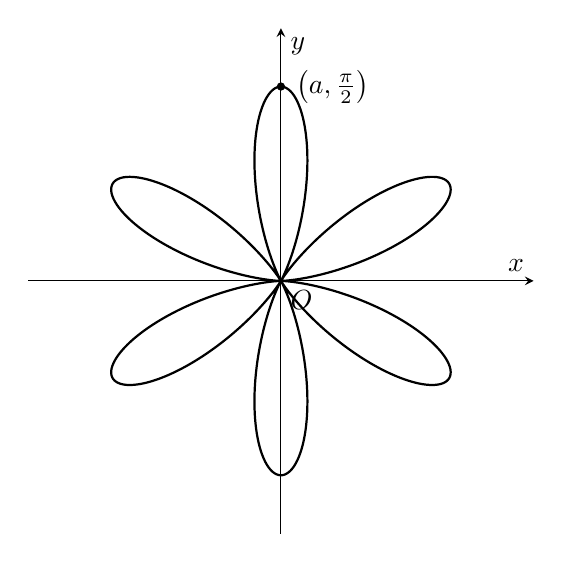
\begin{tikzpicture}
\begin{axis}[
  axis lines=middle,
  xlabel={$x$},
  ylabel={$y$},
  width=0.75\linewidth,
  height=8cm,
  xmin=-1.3, xmax=1.3,
  ymin=-1.3, ymax=1.3,
  ticks=none,
  enlargelimits=false,
  axis equal image,
  clip mode=individual
]
\addplot[
  domain=0:360,
  samples=600,
  smooth,
  thick
]
({(sin(3*x))^2*cos(x)},{(sin(3*x))^2*sin(x)});
\coordinate (Top) at (axis cs:0,1);
\fill (Top) circle (1.5pt);
\node[right, xshift=2pt] at (Top) {$\left(a,\frac{\pi}{2}\right)$};
\node[below right] at (axis cs:0,0) {$O$};
\end{axis}
\end{tikzpicture}} & & \\
& \msFeature{Shape} & B1 & {Six closed petals of equal size, each meeting the pole, with no part of the curve elsewhere.} \\
& \msFeature{Labelled point} & B1 & {Petals centred on \(\theta = \frac{\pi}{6} + \frac{k\pi}{3}\), one along each direction of the \(y\)-axis, with \(r = a\) marked at a tip.} \\
\nopagebreak & & [2] & \\
10(b) & {\(\tfrac12\int_0^{\pi/3} a^2\sin^4 3\theta\,\mathrm{d}\theta\)} & B1 & {Limits for one petal, or \(0\) to \(2\pi\), or other limits with the matching multiple; needs \(\frac12\) and \(a^2\).} \\
& {\(\sin^4 3\theta = \left(\frac{1 - \cos 6\theta}{2}\right)^2\)\\[4pt] \(\phantom{\sin^4 3\theta} = \frac14\left(1 - 2\cos 6\theta + \frac{1 + \cos 12\theta}{2}\right)\)} & M1 & {Uses a double-angle identity twice, or any valid method, to reach a constant and terms in \(\cos 6\theta\) and \(\cos 12\theta\); condone coefficient slips.} \\
& {\(\sin^4 3\theta = \frac18\left(3 - 4\cos 6\theta + \cos 12\theta\right)\)} & A1 & {oe, including within the integrand.} \\
& {\(\frac{a^2}{16}\left[3\theta - \frac23\sin 6\theta + \frac1{12}\sin 12\theta\right]\)} & M1 & {Integrates their \(p + q\cos 6\theta + s\cos 12\theta\) to the form \(\alpha\theta + \beta\sin 6\theta + \gamma\sin 12\theta\).} \\
& {\(6 \times \frac{a^2}{16}\left[3 \times \frac{\pi}{3} - 0 + 0\right]\)} & dM1 & {Substitutes their limits and multiplies by the number of copies those limits need (6 for one petal, 1 for \(0\) to \(2\pi\)).} \\
& {\(\frac{3\pi a^2}{8}\)} & A1 & {cso, oe.} \\
\nopagebreak & & [6] & \\
\nopagebreak \SetCell[c=2]{r} Total for Question 10 & & 8 & \\
\end{msscheme}

\msQuestion{11}
\begin{msscheme}{
  hline{3-16} = {2-Z}{0.4pt, msGrid},
  hline{17} = {0.4pt, msGrid},
  cell{9-16}{2-4} = {bg=msTint},
  row{17} = {font=\bfseries},
}
Question & Scheme & Marks & Notes \\
11 & {\((1 + 2\sin\theta)\sin\theta = 1\)\\[4pt] \(\Rightarrow 2\sin^2\theta + \sin\theta - 1 = 0\)\\[4pt] \(\Rightarrow \sin\theta = \ldots\)} & M1 & {Sets \(r\sin\theta = 1\) with \(r = 1 + 2\sin\theta\), forms a three-term quadratic in \(\sin\theta\) and solves it by any means, calculator allowed.} \\
& {\(\theta = \frac{\pi}{6}\)} & A1 & {Condone \(\sin\theta = -1\) not explicitly rejected.} \\
& {\(\tfrac12\int_{\pi/6}^{\pi/2}(1 + 2\sin\theta)^2\,\mathrm{d}\theta\)} & B1 & {Limits may first be seen when substituted.} \\
& {\(= \tfrac12\int(3 + 4\sin\theta - 2\cos 2\theta)\,\mathrm{d}\theta\)\\[4pt] \(\phantom{=} = \tfrac12\left[3\theta - 4\cos\theta - \sin 2\theta\right]\)} & M1 & {Expands \((1 + 2\sin\theta)^2\) to three terms, uses \(\sin^2\theta = \frac12(1 \pm \cos 2\theta)\) and integrates, at least one trigonometric term correct. Condone coefficient slips.} \\
& {\(\tfrac12\left[\tfrac{3\pi}{2} - \left(\tfrac{\pi}{2} - 2\sqrt3 - \tfrac{\sqrt3}{2}\right)\right]\)\\[4pt] \([= \tfrac{\pi}{2} + \tfrac{5\sqrt3}{4}]\)} & dM1 & {Substitutes \(\frac{\pi}{2}\) and their \(\theta\) at \(A\) into their integrated expression and subtracts, upper minus lower.} \\
& {Triangle \(ONA = \tfrac12 \times 1 \times \sqrt3 = \tfrac{\sqrt3}{2}\)} & B1 & \\
& {\(\text{Area} = \tfrac{\pi}{2} + \tfrac{5\sqrt3}{4} - \tfrac{\sqrt3}{2}\)\\[4pt] \(\phantom{\text{Area}} = \tfrac{\pi}{2} + \tfrac{3\sqrt3}{4}\)} & A1 & {cso. Any exact equivalent, such as \(\frac{2\pi + 3\sqrt3}{4}\).} \\
& \SetCell[c=3]{l} \msAlternative{Area between the curve and \(r = \operatorname{cosec}\theta\)} & & \\
\nopagebreak & {\((1 + 2\sin\theta)\sin\theta = 1\)\\[4pt] \(\Rightarrow 2\sin^2\theta + \sin\theta - 1 = 0\)\\[4pt] \(\Rightarrow \sin\theta = \ldots\)} & M1 & {Sets \(r\sin\theta = 1\) with \(r = 1 + 2\sin\theta\), forms a three-term quadratic in \(\sin\theta\) and solves it by any means, calculator allowed.} \\
& {\(\theta = \frac{\pi}{6}\)} & A1 & {Condone \(\sin\theta = -1\) not explicitly rejected.} \\
& {\(r\sin\theta = 1 \Rightarrow r = \operatorname{cosec}\theta\)} & B1 & {Or \(r = \frac{1}{\sin\theta}\).} \\
& {\(\text{Area} = \tfrac12\int_{\pi/6}^{\pi/2}\left[(1 + 2\sin\theta)^2 - \operatorname{cosec}^2\theta\right]\,\mathrm{d}\theta\)\\[4pt] \(= \tfrac12\int(3 + 4\sin\theta - 2\cos 2\theta - \operatorname{cosec}^2\theta)\,\mathrm{d}\theta\)} & M1 & {Uses \(\frac12\int\) of \((1 + 2\sin\theta)^2\) minus the square of their \(r\) for \(AN\), expands, uses \(\sin^2\theta = \frac12(1 \pm \cos 2\theta)\) and integrates at least one trigonometric term correctly.} \\
& {\(= \tfrac12\left[3\theta - 4\cos\theta - \sin 2\theta + \cot\theta\right]\)} & A1 & {All four terms correct; the \(\frac12\) may be applied later.} \\
& {\(\tfrac12\left[\tfrac{3\pi}{2} - \left(\tfrac{\pi}{2} - \tfrac{5\sqrt3}{2} + \sqrt3\right)\right]\)} & dM1 & {Substitutes \(\frac{\pi}{2}\) and their \(\theta\) at \(A\) into their integrated expression and subtracts, upper minus lower.} \\
& {\(= \tfrac{\pi}{2} + \tfrac{3\sqrt3}{4}\)} & A1 & {cso. Any exact equivalent, such as \(\frac{2\pi + 3\sqrt3}{4}\).} \\
\nopagebreak \SetCell[c=2]{r} Total for Question 11 & & 7 & \\
\end{msscheme}

\msQuestion{12}
\begin{msscheme}{
  hline{3-7,9-14} = {2-Z}{0.4pt, msGrid},
  hline{8,15} = {0.4pt, msGrid},
  row{15} = {font=\bfseries},
}
Question & Scheme & Marks & Notes \\
12(a) & \SetCell[c=3]{c} \msFigure{\begin{tikzpicture}
 \begin{axis}[
width=0.75\linewidth,
height=8cm,
axis lines=middle,
axis equal image,
xmin=-3.9, xmax=1.3,
ymin=-2.2, ymax=2.2,
xlabel={$x$},
ylabel={$y$},
xtick=\empty,
ytick=\empty,
clip mode=individual
 ]
 \addplot[
thick,
smooth,
samples=300,
domain=0:360,
variable=\t
 ]
 (
{sqrt((pi^2-((\t*pi/180)-pi)^2)/(1+((\t*pi/180)-pi)^2))*cos(\t)},
{sqrt((pi^2-((\t*pi/180)-pi)^2)/(1+((\t*pi/180)-pi)^2))*sin(\t)}
 );
 \coordinate (Far) at (axis cs:-pi,0);
 \fill (Far) circle (1.5pt);
 \node[above left] at (Far) {$(\pi,\pi)$};
 \node[below left] at (axis cs:0,0) {$O$};
 \end{axis}
 \end{tikzpicture}} & & \\
& \msFeature{Shape} & B1 & {One closed loop through the pole, lying mainly on the \(\theta = \pi\) side of it, symmetric about the initial line.} \\
& \msFeature{Intercepts} & B1 & {Both ends of the curve at the pole. Condone the tangent there not along the initial line.} \\
& {\(\theta = \pi\): \(r^2 = \frac{\pi^2 - 0}{1 + 0} \Rightarrow r = \ldots\)} & M1 & {Substitutes \(\theta = \pi\) into the equation to find \(r\). No justification that this is the furthest point is needed.} \\
& {\((\pi, \pi)\)} & A1 & {Or \(r = \pi\) and \(\theta = \pi\) stated.} \\
\nopagebreak & & [4] & \\
12(b) & {\(A = \frac12\int_0^{2\pi}\frac{\pi^2 - (\theta - \pi)^2}{1 + (\theta - \pi)^2}\,\mathrm{d}\theta\)} & B1 & {\(\frac12\), \(r^2\) substituted and limits \(0\), \(2\pi\); or \(\int_0^{\pi}\) of \(r^2\) by symmetry.} \\
& {\(u = \theta - \pi\):\\[4pt] \(\frac{\pi^2 - u^2}{1 + u^2} = -1 + \frac{\ldots}{1 + u^2}\)} & M1 & {Replaces \(\theta - \pi\) by \(u\) and writes the integrand as \(a + \frac{b}{1 + u^2}\), by division or otherwise. Condone wrong \(a\) and \(b\).} \\
& {\(A = \frac12\int_{-\pi}^{\pi}\left(-1 + \frac{\pi^2 + 1}{1 + u^2}\right)\,\mathrm{d}u\)} & A1 & {Correct integrand with limits \(\pm\pi\), oe, such as \(\int_0^{\pi}\) without the \(\frac12\). Limits \(0\), \(2\pi\) with a \(u\) integrand is A0.} \\
& {\(\phantom{A} = \frac12\left[-u + (\pi^2 + 1)\arctan u\right]_{-\pi}^{\pi}\)} & M1 & {Integrates their \(a + \frac{b}{1 + u^2}\) to \(au + b\arctan u\). Condone wrong \(a\) and \(b\).} \\
& {\(\frac12\left[\left(-\pi + (\pi^2 + 1)\arctan\pi\right)\right.\)\\[4pt] \(\phantom{\frac12[}\left.{}- \left(\pi - (\pi^2 + 1)\arctan\pi\right)\right]\)} & dM1 & {Substitutes the limits of their correctly transformed full or half interval into their antiderivative, subtracts and applies any required symmetry factor.} \\
& {\(A = (\pi^2 + 1)\arctan\pi - \pi\)} & A1 & {oe, such as \((\pi^2 + 1)\tan^{-1}\pi - \pi\). cso.} \\
\nopagebreak & & [6] & \\
\nopagebreak \SetCell[c=2]{r} Total for Question 12 & & 10 & \\
\end{msscheme}

\end{document}
